\chapter{Proposta para análise de arquiteturas \ac{mmorpg}}
\label{cap3}

\section{Proposta}
\label{proposta}



Este trabalho propôe-se a realizar a análise de consumo de recursos por arquiteturas de microsserviços para jogos \ac{mmorpg}.
%
Para este fim, o atual trabalho usará uma arquitetura para análise disponíveis na literatura a fim de encontrar gargalos nestas arquiteturas.



Para obter dados a fim de efetuar uma análise do uso de recursos computacionais consumidos por arquiteturas de jogos \ac{mmorpg}, se faz necessário a execução do plano de testes.
%
Os critérios serão abordados na Seção~\ref{analise}.
%
O plano de testes irá analisar os seguintes aspéctos nas arquiteturas:



\begin{enumerate}
\item Consumo de memória: Análise do consumo de memória do sistema levando em consideração o número de conexões.
\item Consumo de memória secundária: Análise do consumo de memória secundária para funcionamento dos microsserviços tanto do banco de dados.
\item Consumo de CPU: Análise do consumo de processamento, tanto em relação ao tempo de resposta das requisições quanto ao consumo obtido do sistema operacional.
\item Consumo de Banda: Análise da vasão de dados com relação ao número de conexões em que cada microsserviço será submetido.
\end{enumerate}



A análise será realizada capturando informações sobre o uso de recursos do sistema operacional que implantará a base das arquiteturas, obtendo assim estes dados de forma gráfica para que auxiliem a análise.
%
Os recursos analisados são memória, memória secundária, processador, banda e número máximo de conexões.
%
Tais dados coletados permitirão tomadas de decisão de projetos para o desenvolvimento de jogos \ac{mmorpg}.
%
Este plano de testes será abordado na Seção~\ref{testes}.



A execução do plano testes usará uma arquitetura disponível na literatura.
%
Entretanto, existem algumas abordagens diferentes no desenvolvimento de tais arquiteturas.
%
Por este motivo, é necessário descrever as arquiteturas existentes na literatura.



\subsection{Rudy}

A arquitetura Rudy~\cite{matthiasrudy2011} tem como objetivo criar multiplos mundos isolados, na qual cada microsserviço será responsável por um mundo.
%
Esta arquitetura pode ser visualizada na Figura~\ref{rudy}.


\begin{figure}[htb!]
  \caption{Arquitetura Rudy.}
  \label{rudy}
  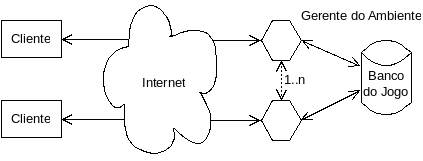
\includegraphics[height=3.5cm]{img/cap3/rudy.png}
  \centering

  Adaptado de:~\cite{matthiasrudy2011}.
\end{figure}

O banco de dados de armazenamento de estado de mundo é compartilhado na arquitetura Rudy (Figura~\ref{rudy}), porém pode não ter ligação lógica entre cada mundo no banco.
%
Esta arquitetura é escalável, porém é limitada o número de conexões em um único ambiente.



O gerente de ambiente por sua vez será comunicado via \ac{tcp}.
%
O funcionamento interno desta arquitetura trabalhará em rodadas.
%
Cada jogador pode enfileirar somente um número determinado de requisições para ser consumido pelo ciclo de processamento do gerente de ambiente.
%
Por sua vez, o consumidor de requisições irá atualizar o estado no mundo e enviar o resultado, caso a requisição tenha uma resposta.
%
O modelo de processamento do gerente de ambiente pode ser visualizado na Figura~\ref{fig:processamento}.



\begin{figure}[htb!]
  \caption{Modelo de \textit{Threads} do gerente de ambiente.}
  \label{fig:processamento}
  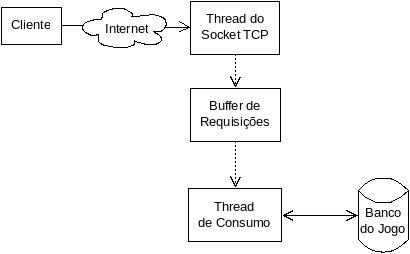
\includegraphics[height=4.5cm]{img/cap3/thread_model.png}
  \centering

  Adaptado de:~\cite{matthiasrudy2011}.
\end{figure}

O mesmo modelo de processamento paralelo apresentado na Figura~\ref{fig:processamento} para consumo das requisições dos clientes é utilizado de forma similar na arquitetura Willson (Seção~\ref{willson}) e Salz (Seção~\ref{salz}).


\subsection{Salz}
\label{salz}



A arquitetura Salz~\cite{albion_online_unite} tem como objetivo criar um único mundo, integrando mais jogadores no mesmo ambiente.
%
A sua estratégia de escalabilidade está na divisão do ambiente em \textit{chunks}, diminuindo o impacto do número de conexões em casos onde a comunidade está esparsa pelo ambiente.
%
Entretanto, esta arquitetura contém problemas com relação a aglomeração da comunidade, visto que a relação a pedaços do ambiente está diretamente relacionada ao poder computacional para processamento do mesmo.
%
Nesse sentido, torna-se viavel o uso desta arquitetura para jogos onde a frequência de jogadores na mesma região é baixa.
%
Ela é visível na Figura~\ref{fig:salz}.


\begin{figure}[htb!]
  \caption{Arquitetura Salz.}
  \label{fig:salz}
  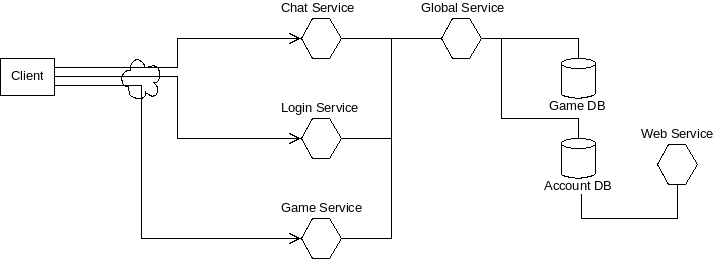
\includegraphics[height=3cm]{img/cap3/salz.png}
  \centering

  Adaptado de:~\cite{albion_online_unite}.
\end{figure}


O microsserviço de gerenciamento de cenário tratará as requisições utilizando o mesmo modelo de processamento paralelo descrito na Figura~\ref{fig:processamento}, na qual recebe as requisições comunicadas através do protocolo \ac{tcp}, realizando as alterações no cenário a qual cada microsserviço é responsável.
%
A sua principal diferença está na certeza de que o banco de dados é compartilhado entre todos os microsserviços, e periodicamente atualiza os dados salvos em memória ao banco de dados físico, também atualizando durante a desconexão ou miração entre serviços do personagem.



\subsection{Willson}
\label{willson}

A arquitetura Willson~\cite{stephenclarkewillson2017} (Figura~\ref{fig:willson}) tenta suprir a necessidade de migração de conexão entre microsserviços ao personagem transladar dentre \textit{chunks} distintos.
%
Dessa forma, a arquitetura deixa de armazenar a estrutura da cena em memória para armazenar os status de objetos do ambiente em um banco de dados em memória compartilhado.
%
Nesse sentido, o ambiente torna-se escalável, porém é limitado ao desempenho do banco de dados escolhido.
%
Esta arquitetura permite implantar microsserviços sem configurações individuais, na qual facilita a sua gestão de manutenção e distribuição de carga.

\begin{figure}[htb!]
  \caption{Arquitetura Salz.}
  \label{fig:willson}
  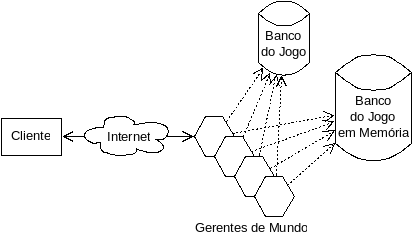
\includegraphics[height=4.5cm]{img/cap3/willson.png}
  \centering

  Adaptado de:~\cite{albion_online_unite}.
\end{figure}

O processamento de requisições segue o modelo de processamento paralelo descrito na Figura~\ref{fig:processamento}.
%
Entretanto, este serviço não armazenará nada em sua memória, realizando todas as operações no banco do jogo em memória.


\section{Critérios de análise}
\label{analise}

A etapa de análise das arquiteturas descritas na proposta (Seção~\ref{proposta}) busca gerar informações que ajudem a compreender o consumo de recursos das arquiteturas de microsserviços.
%
A análise terá escopo limitado, ignorando a orquestração de microsserviços, balanço de carga e serviços sociais/econômicos destas arquiteturas, focando somente na gerência do ambiente do jogo.
%
A proposta atual pretende analisar seguindo os seguintes critérios:

\begin{enumerate}
  \item Consumo de recursos por conexão: Será analisado o comportamento dos recursos utilizados comparado ao número de conexões ativas no ambiente, a fim de analisar a escalabilidade destes sistemas. Analisar em específico os recursos de memória principal, memória secundária, processamento, largura de banda da rede. e tempo para processar uma requisição
  \item Limite de conexões por arquitetura: Comparar o limite de conexões com um recurso alocado finito, a fim de validar o consumo de recursos pela arquitetura. Analisar em específico os recursos de memória principal, memória secundária, processamento e largura de banda da rede e tempo para processar uma requisição.
\end{enumerate}

\section{Plano de testes}
\label{testes}
